\documentclass[final,pdftex]{../../template/epsilonj}

\RequirePackage{graphicx}
\RequirePackage[colorlinks,citecolor=blue,urlcolor=blue]{hyperref}

\usepackage{colortbl}
\definecolor{rrow}{rgb}{1,0.9,1}
\definecolor{ccol}{rgb}{1,1,0.6}
\definecolor{inters}{rgb}{1,0.9,0.6}

\addbibresource{../../template/epsilon.bib}

\begin{document}
\setcounter{page}{15}

	% \microtypesetup{protrusion=false, expansion=false}
	\begin{frontmatter}
		\title{Как выбрать функциональную форму уравнения регрессии}
		\runtitle{Как выбрать функциональную форму уравнения регрессии}
		
		\begin{aug}
			\author{\imya{Кирилл} \fam{Фурманов}}
			\runauthor{Фурманов К. К.}
			\address{Кафедра математической экономики и~эконометрики, НИУ ВШЭ, Москва.}
		\end{aug}
		
		\begin{abstract}
			Аннотация должна передавать краткое содержание работы.
			Она должна быть ясной, содержательной, релевантной и~короткой
			(не более 150~слов). Аннотация должна содержать информацию,
			необходимую для поиска по базам научных работ.
			В~аннотации не должно быть математических формул.
		\end{abstract}
		
		\begin{keyword}
			\kwd{функциональная форма}
			\kwd{диагностика остатков}
			\kwd{нормальность остатков}
		\end{keyword}
		
	\end{frontmatter}
	

Если человек, начинающий изучать статистику, задаст вопрос, что же такое регрессионный анализ и~чем он отличается от анализа корреляционного, он может получить такой ответ: и~то и~другое связано с~изучением статистических связей, но задача корреляционного анализа "--- измерение тесноты связи между признаками, а~задача регрессионного анализа "--- определение формы этой связи. По мере продолжения обучения этот человек начнёт, вероятно, подозревать, что форма связи практически одна "--- линейная. Иногда какие"=нибудь переменные логарифмируются "--- то ли для разнообразия, то ли для приличия.

Более того, изучение статей с~применением регрессионных моделей может подтвердить эти подозрения. В~них исследователи излагают истории своей борьбы с~гетероскедастичностью, мультиколлинеарностью, эндогенностью, но редко внимание сосредотачивается на определении функциональной формы зависимости. И~даже когда встречаются существенно нелинейные модели, часто остаётся вопрос: почему у~зависимости именно такой вид? Кажется, они приходят авторам откуда"=то свыше "--- с~потолка, что ли.

А~ведь задача определения вида функции регрессии "--- самая существенная, если отрешиться от содержательной стороны дела и~рассматривать только статистические проблемы. Все статистические выводы имеют смысл, только если форма зависимости выбрана правильно "--- без этого сомнительна польза дальнейших изысканий, не спасают ни бутстрап, ни самый обобщённый метод моментов.

Итак, есть повод задуматься над двумя вопросами. Первый: как определить функциональную форму зависимости? Второй: почему так популярны линейные и~линейные в~логарифмах модели? Должно быть, когда"=то они были популярны из-за простоты, но сейчас нет особых проблем в~подгонке нелинейных зависимостей: процедуры подгонки реализованы в~доступных статистических программах.

Пока что оставим эти вопросы читателю на обдумывание и~возьмёмся за проблему с~другого конца. Давайте сначала представим, что у~нас уже есть полностью специфицированное уравнение регрессии. Более того, оно уже оценено, и~теперь стоит вопрос: было ли оно правильным? Может, мы пытались подогнать линейную зависимость под данные, порождённые нелинейным процессом? Может, мы прологарифмировали все переменные, хотя в~этом не было нужды? Как это выяснить?

\section{Визуальная диагностика}

Если оценивается парная регрессия, ответ очевиден: нужно построить график (пожалуй, это стоило сделать ещё до оценивания). По диаграмме рассеяния часто легко догадаться, какую зависимость стоит подгонять. Может быть, график нас всё же смущает "--- например, там недостаточно наблюдений, чтобы уверенно сделать выбор. Тогда на помощь полезно призвать теорию изучаемого явления, устоявшиеся традиции моделирования и~здравый смысл. Если и~это не помогло, стоит выбрать вариант попроще. Кроме того, если у~нас есть две модели, из которых сложно выбрать одну, то мы можем сравнить выводы, полученные из обеих. Если они схожи "--- прекрасно, не надо и~выбирать. Если они различаются, то мы хотя бы знаем, насколько результаты зависят от выбора модели.

Для множественной регрессии уже не получится на одном графике представить все переменные, но унывать не стоит. Есть несколько полезных способов проверки выбранной функциональной формы.

\subsection{График «остатки "--- прогнозы»}

После оценивания модели постройте график зависимости остатков от модельных (прогнозных) значений объясняемой величины. В~идеальном случае график не выявит никакой зависимости (см. рис.~\ref{fig:res-fitted-correct}). При правильной спецификации остатки должны вести себя беспорядочно "--- если мы обнаружим какую"=то связь между прогнозными значениями и~остатками, то её можно использовать для улучшения функциональной формы. На рис.~\ref{fig:res-fitted-omitted} показан пример графика, полученного при подгонке линейной зависимости под данные, порождённые квадратичной моделью $y = \beta_1 + \beta_2 x + \beta_3 x^2 + \e$. Видно, что остатки разбросаны вдоль параболы. Для усиления наглядности можно дополнить график сглаженной зависимостью остатков от прогнозов "--- линией, полученной методом lowess или ядерной регрессией. Можно вместо остатков откладывать по вертикальной оси наблюдаемые значения объясняемой переменной "--- тогда в~идеальном случае график будет выглядеть как облако точек, рассеянное вдоль биссектрисы прямого угла "--- линии $y = \hat y$.

\begin{figure}[hbtp]
	\centering
	\subfigure[{Верная спецификация}]{%
		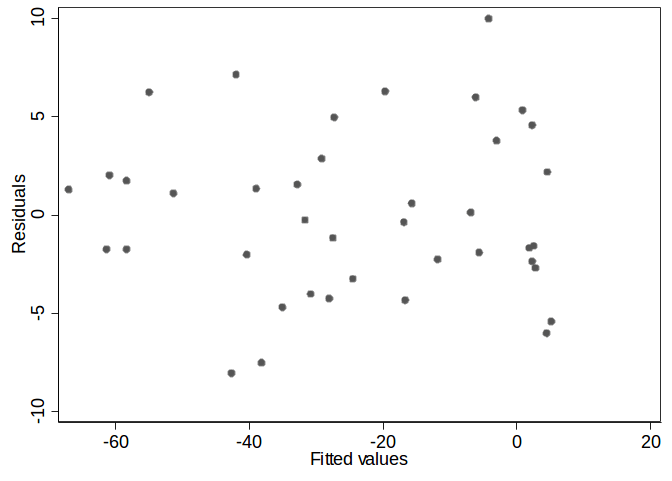
\includegraphics[width=5.5cm]{res-fitted-correct.png}
		\label{fig:res-fitted-correct}} \quad
	\subfigure[{Пропущенный квадратичный член}]{%
		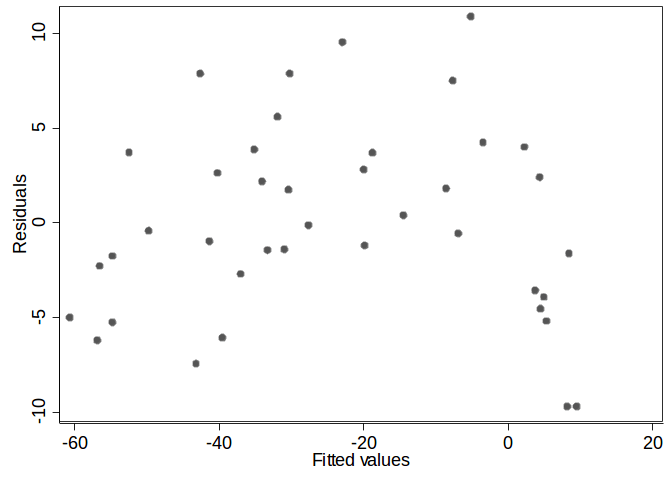
\includegraphics[width=5.5cm]{res-fitted-omitted.png}
		\label{fig:res-fitted-omitted}} 
	\caption{График «остатки "--- прогнозы» при пропуске переменной}
\end{figure}

Есть также смысл смотреть на график зависимости остатков от каждого из регрессоров: это может натолкнуть на мысль, гд\'{е} именно кроется ошибка. Стоит только помнить об~опасности множественных проверок: при большом количестве объясняющих переменных график для какой"=нибудь из них может оказаться подозрительным просто по случайности.

Часто на графике «остатки "--- прогнозы» отражается не только рассеяние остатков вдоль кривой, но и~усиление или уменьшение их разброса. Рис.~\ref{fig:res-fitted-wrong} соответствует случаю, в~котором линейная модель $y = \beta_1 + \beta_2 x + \e$ подгонялась под данные, порождённые логарифмической моделью $\ln y = \beta_1 + \beta_2 \ln x + \e$. Стоит отличать этот случай от того, в~котором остатки имеют непостоянный разброс, но при этом рассеяны вдоль прямой "--- горизонтальной оси (рис.~\ref{fig:res-fitted-het}). Изменение разброса без изменения среднего уровня остатков свидетельствует о~гетероскедастичности (непостоянстве дисперсии случайной составляющей), а~не об~ошибке функциональной формы. Это тоже проблема, но последствия и~способы решения у~неё другие.

\begin{figure}[htbp]
	\centering
	\subfigure[{Неверная функциональная форма}]{%
		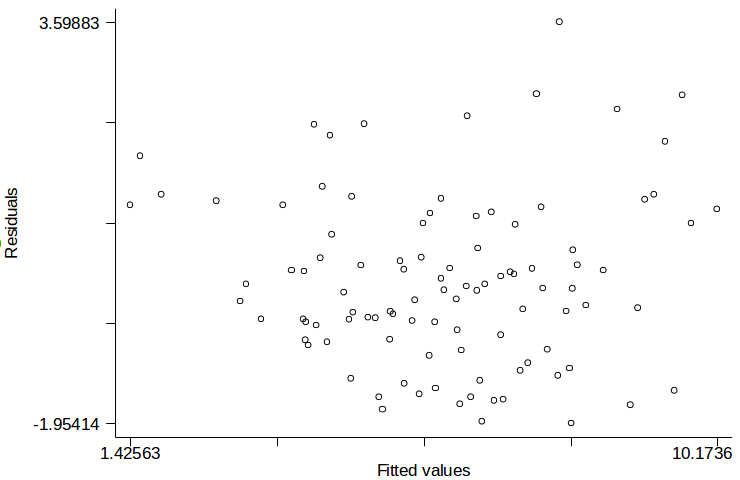
\includegraphics[width=5.5cm]{res-fitted-wrong.png}
		\label{fig:res-fitted-wrong}} \quad
	\subfigure[{Гетероскедастичность}]{%
		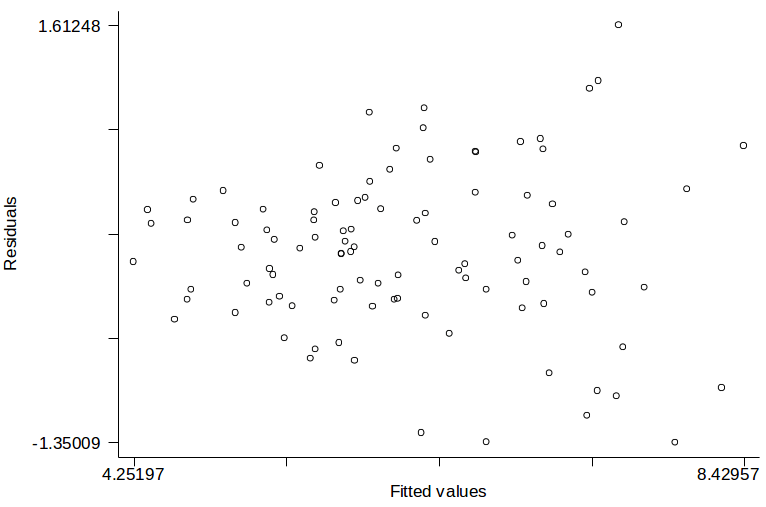
\includegraphics[width=5.5cm]{res-fitted-het.png}
		\label{fig:res-fitted-het}} 
	\caption{График «остатки "--- прогнозы» при непостоянном разбросе}\label{fig:wrong}
\end{figure}

Возможно, посмотрев на рис.~\ref{fig:wrong}, вы не найдёте явных различий между двумя графиками. Увы, понять, чем же именно грешит оценённая модель, часто нелегко.

Основной недостаток всех визуальных тестов "--- это то, что результат зависит от воображения смотрящего. Посмотрите на отсканированный лист из экзаменационной работы по эконометрике Дмитрия Арсютина (рис.~\ref{fig:interpretation}). Отмеченные экзаменуемым проблемные явления вовсе не были задуманы автором задания; не заметил их и~никто другой из студентов, писавших тот же экзамен.

\begin{figure}[htbp]
	\centering
	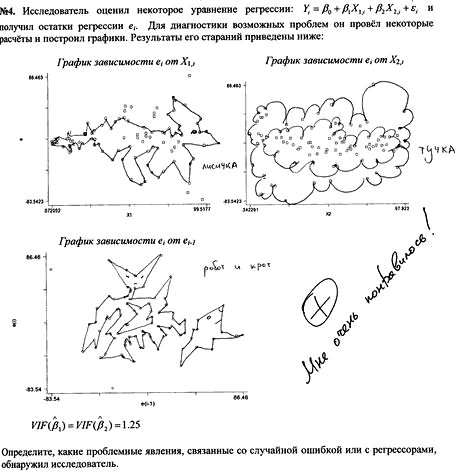
\includegraphics[width=8cm]{interpretation.png}
	\caption{Пример вольной интерпретации графика «остатки "--- прогнозы».}\label{fig:interpretation}
\end{figure} 

\section{Диагностические тесты}

\subsection{Тест Рамсея}

Он же RESET "--- Regression Equation Specification Error Test\footnote{В~статье \citet{ramsey69} можно ещё почитать про три теста с~названиями RASET, KOMSET и~BAMSET.}\fnnsp. Рассчитайте несколько степеней прогнозных значений $\hat y$ и~проверьте, не улучшает ли результат их включение в изначальную модель. Например, можно включить квадрат и~куб прогнозов:
\[
y = \beta_1 + \beta_2 x + \ldots + \beta_k x_k + \gamma_2 \hat y^2 + \gamma_3 \hat y^3 + \e
\]

Если первоначальная модель верно специфицирована, то добавленные нелинейные члены должны быть незначимы, что соответствует основной гипотезе теста.
\[
\hypo_0\colon \gamma_2 = \gamma_3 = 0, \quad \hypo_A\colon \gamma_2^2 + \gamma_3^2 > 0 \text{ (ошибка спецификации).}
\]

Это гипотеза о~линейном ограничении, которая проверяется обычной $\Fish$"~статистикой. Выбор числа степеней прогнозов $\hat y$ остаётся за исследователем.

Результаты теста Рамсея не зависят от воображения, но куда менее информативны, чем график. При выявленной ошибке они не дают подсказки, какую функциональную форму стоит выбрать и~насколько сильно отклонение от первоначально оценённой зависимости. При большом числе наблюдений основная гипотеза может отвергаться и~в~том случае, когда обнаруженная ошибка спецификации незначительна, так что вы, возможно, предпочли бы ей пренебречь («ловушка большой выборки»). Это касается и~другого популярного способа проверки функциональной формы "--- теста Бокса"--~Кокса\footnote{Статья"=первоисточник \citep{boxcox64} может оказаться нелёгким чтивом, но можно ознакомиться с~сутью преобразования Бокса"--~Кокса и~его использованием для определения формы зависимости по работе \citet{sakia92}.}\fnnsp, "--- да и~любого статистического критерия.

Иногда тест Рамсея называют тестом на пропущенную переменную (\ENGs{omitted variable test}) "--- кажется, это не очень удачное название. Отвержение основной гипотезы не говорит о~необходимости добавлять в~модель \textit{содержательно новую} переменную, отражающую неучтённый статистический признак. Речь, скорее, о~том, что функциональная форма может исправиться при включении в~модель преобразованных значений тех величин, что уже есть в~уравнении "--- например, добавлении квадрата или логарифма какого"=либо регрессора.

\subsection{Проверка нормальности остатков}

По какой"=то причине многие статистики верят, что при правильной спецификации остатки имеют распределение, близкое к~нормальному (исключение "--- модели с~дискретной объясняемой переменной и~модели времени жизни). Имеет смысл построить для остатков гистограмму или график на вероятностной бумаге. В~некоторых случаях гистограмма может подсказать правильное преобразование переменных в~модели. На рис.~\ref{fig:histqq} изображены гистограмма и~график на вероятностной бумаге (график «квантиль "--- квантиль») для случая, когда линейная зависимость подгонялась вместо логарифмической.

\begin{figure}[htbp]
	\centering
	\subfigure[{Гистограмма}]{%
		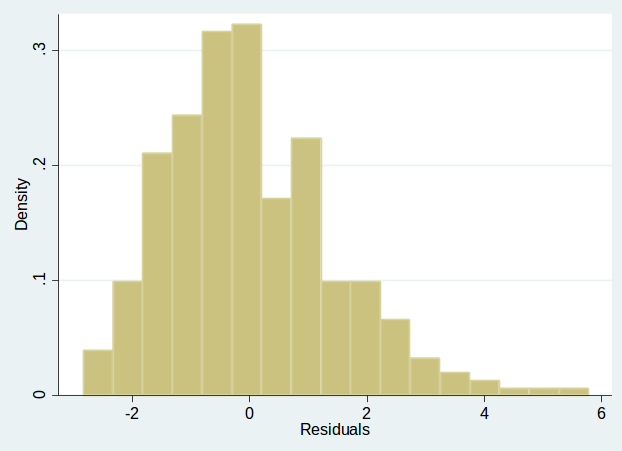
\includegraphics[width=5.5cm]{hist.png}
		\label{fig:hist}} \quad
	\subfigure[{График «квантиль "--- квантиль»}]{%
		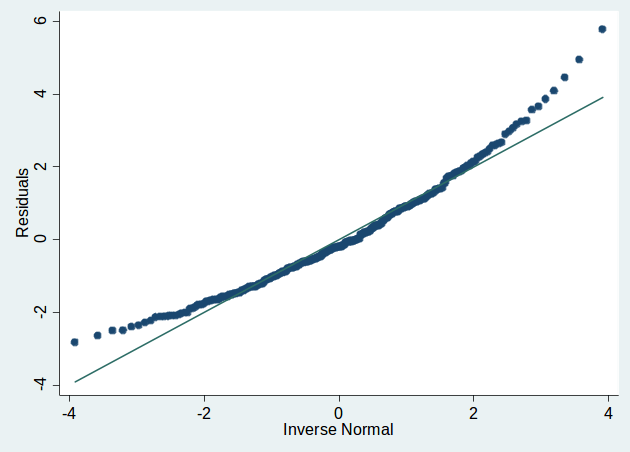
\includegraphics[width=5.5cm]{qq.png}
		\label{fig:qq}} 
	\caption{Распределение остатков при неправильной функциональной форме}\label{fig:histqq}
\end{figure}


К~сожалению, график остатков может искажать не только ошибка спецификации, но и~гетероскедастичность; впрочем, она не должна приводить к~несимметричной гистограмме. От формальных тестов на нормальность (критериев Харке"--~Бера, Шапиро"--~Уилка и~т.\,д.) толку меньше. Они не дают представления о~характере отклонений от нормальности и~могут отвергать основную гипотезу, когда выявленные отклонения не представляются практически значительными.

\section{Функциональная зависимость}

А~теперь вернёмся к~вопросу, с~которого начиналась эта статья: как выбрать функциональную форму? Тесты позволяют понять, нет ли ошибки в~уже оценённом уравнении, но с~какого уравнения разумно начать?

Во-первых, стоит посмотреть, что делали до вас. Для решения многих задач есть уже готовые шаблоны: есть готовые функциональные формы для производственных функций, функций издержек, уравнений заработной платы и~т.\,п. Они могут не подходить идеально для какого"=то конкретного случая, но быть разумной точкой отсчёта.

Во-вторых, стоит подумать. Почему только «во-вторых»? Потому что не стоит слишком полагаться на собственный ум: он иногда подводит. Однако ум (особенно при наличии опыта) может подсказать разумную форму зависимости или хотя бы отбраковать неразумные. Подумайте: могут ли потребление~$C$ и~доход~$Y$ быть связанными уравнением типа $\ln C = \alpha + \beta Y + \e$? Пожалуй, не стоит полагаться на такой вид зависимости, ведь он предполагает, что по мере роста дохода потребление растёт возрастающими темпами (либо падает при $\beta<0$, что не менее странно). Уравнения $C = \alpha + \beta Y + \e$ и~$\ln C = \alpha + \beta \ln Y + \e$ представляются более разумными.

В~предыдущем абзаце как раз перечислены основные формы зависимости в~эконометрике, но, прежде чем рассмотреть их подробнее, вернёмся к~вопросу из начала статьи: почему оцениваются именно линейные зависимости? Можно назвать разные причины, но сейчас рассмотрим такую: параметры линейной модели легко понять. Одна из целей построения статистической модели "--- сведение большого и~трудноосмыслимого объёма данных к~нескольким интерпретируемым параметрам. Если из неосмысливаемого набора чисел в~нашей выборке мы получили неосмысливаемый набор оценок, это может быть вовсе и~не достижением. Именно интерпретируемость делает привлекательными наиболее популярные функциональные формы уравнений регрессии, к~которым мы как раз переходим.

\textit{Линейная} зависимость: $y = \beta_1 + \beta_2 x_2 + \ldots + \beta_k x_k + \e$. Интерпретация коэффициентов такова: увеличение~$x_j$ на единицу соответствует увеличению~$y$ на~$\beta_j$ при прочих равных условиях (то есть при неизменных значениях всех остальных регрессоров и~случайной составляющей). 

\textit{Логарифмическая} зависимость: $\ln y = \beta_1 + \beta_2 \ln x_2 + \ldots + \beta_k \ln x_k + \e$. Увеличение~$x_j$ на один процент приблизительно соответствует увеличению~$y$ на~$\beta_j$ процентов при прочих равных условиях (точнее, в~$1{,}01^{\beta_j}$ раз, но приближение очень хорошее). Иначе говоря, коэффициент $\beta_j$ есть частная эластичность~$y$ по~$x_j$.

\textit{Полулогарифмическая }зависимость: $\ln y = \beta_1 + \beta_2 x_2 + \ldots + \beta_k x_k + \e$. Увеличение $x_j$ на единицу соответствует при прочих равных условиях увеличению~$y$ в~$\ee^{\beta_j}$ раз, или на~$(\ee^{\beta_j}-1)\cdot 100\,\%$. В~этой модели интерпретируются потенцированные коэффициенты, но можно пользоваться тем, что $\ee^{\beta_j} - 1 \sim \beta_j$ по базе $\beta_j \to 0$. Так что если значение коэффициента невелико, то увеличение~$x_j$ на единицу соответствует увеличению~$y$ на $\approx \beta_j \cdot 100\,\%$.

\section{Заключение}

В~заключение статьи "--- пара задач на функциональную форму\footnote{Задачи взяты из задачника \citet{FurmanovZMetr}, который можно найти на странице автора: \url{http://www.hse.ru/org/persons/503346}.}\fnnsp.

\par\medskip

\textbf{Задание №\,1.} Сотрудники НИИ размышляют над тем, как оценивать экспоненциальную зависимость $y$ от $x$. Старший научный сотрудник предлагает свести зависимость к~линейной: $\ln y_i = \beta_1 + \beta_2 x_i + \e_i$ "--- и~оценить её с~помощью МНК. Его молодой коллега предлагает применить метод максимального правдоподобия для оценивания нелинейной модели $y_i \sim \mathcal{N} (\mu_i, \sigma^2)$, $\mu_i = \exp(\beta_1 + \beta_2 x_i)$. Посмотрите на две возможные диаграммы рассеяния признаков $y$ и~$x$ (рис.~\ref{fig:diag}). Скажите, в~каком случае вы бы поддержали старшего, а~в~каком "--- младшего научного сотрудника.

\begin{figure}[htbp]
	\centering
	\subfigure[{Рассеяние~1}]{%
		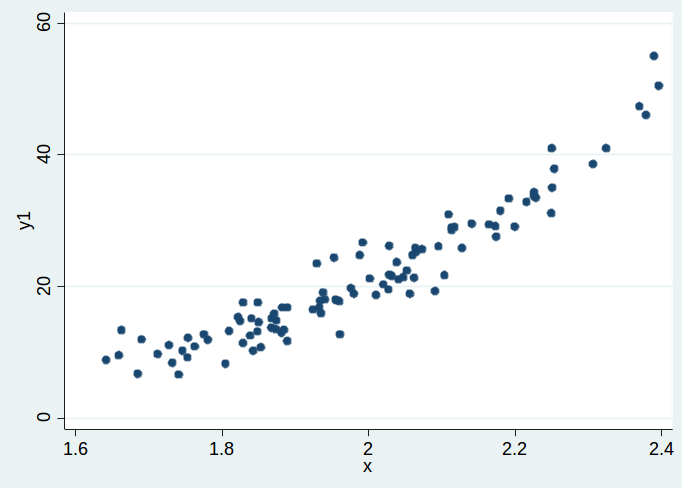
\includegraphics[width=5.5cm]{nii1.png}
		\label{fig:nii1}} \quad
	\subfigure[{Рассеяние~2}]{%
		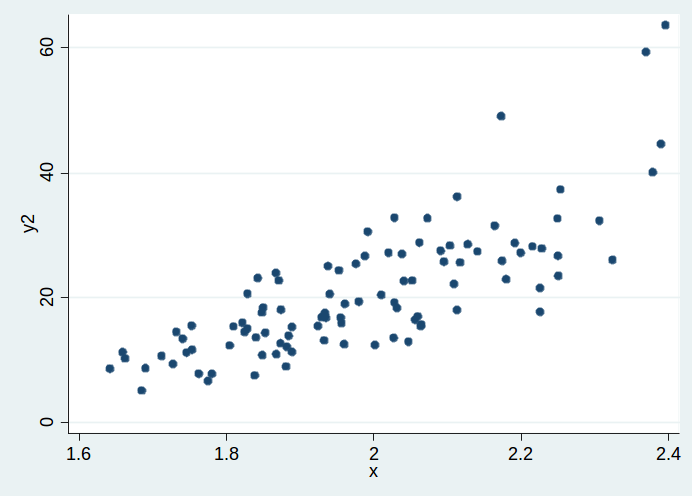
\includegraphics[width=5.5cm]{nii2.png}
		\label{fig:nii2}} 
	\caption{Диаграммы к~заданию 1}\label{fig:diag}
\end{figure}


\textbf{Задание №\,2.} Однажды любознательные барышни Оля и~Маша оценили зависимость $y_i = \beta_1 + \beta_2 x_i + \e_i$. Оля провела тест, выявивший наличие гетероскедастичности. Маша решила, что результаты теста могут быть следствием ошибки спецификации. Оля, чтобы одолеть гетероскедастичность, оценила модель $\frac{y_i}{\sqrt{x_i}} = \alpha_1 \frac{1}{\sqrt{x_i}} + \alpha_2 \sqrt{x_i} + \nu_i$. Маша, чтобы устранить ошибку спецификации, перешла к~логарифмам: $\ln y_i = \gamma_1 + \gamma_2 \ln x_i + u_i$. И~тот, и~другой подход дали хорошие результаты: в~новых моделях тесты не выявили ни гетероскедастичности, ни ошибки спецификации. Представьте себя на месте любознательных барышень: какими соображениями вы бы руководствовались при выборе одной из этих двух моделей?

\textit{Автор говорит спасибо Дмитрию Арсютину, без чьей работы эта статья была бы беднее.}

\nocite{sakia92}	

\printbibliography	
	
\end{document}

